\documentclass{article}
\usepackage{amsmath}

\usepackage[none]{hyphenat}                                                                                                              
\usepackage{helvet}
\renewcommand{\familydefault}{phv}

\makeatletter
\renewcommand{\normalsize}{\@setfontsize\normalsize{6}{6.5}}
\makeatother

\usepackage{tikz}
\usetikzlibrary{shapes,calc,patterns}

\definecolor{red}{rgb}{0.79, 0.00, 0.01} % 201/0/3
\definecolor{blue}{rgb}{0.12, 0.43, 0.59} % 30/110/150
\definecolor{mdslate}{rgb}{0.45, 0.50, 0.68} % 114/127/173
\definecolor{ltslate}{rgb}{0.75, 0.80, 0.98} % 216/225/229

\colorlet{colbox}{ltslate}
\tikzstyle{domainstyle}=[fill=colbox,opacity=0.4,draw=black,line join=round,shade]
\tikzstyle{domainshade}=[top color=mdslate,bottom color=ltslate]
\tikzstyle{coordsys}=[color=gray,line width=0.5pt]
\tikzstyle{dimension}=[color=blue,line width=0.5pt]
\tikzstyle{dispbc}=[color=red,line width=1.0pt]
\tikzstyle{ground}=[color=gray,fill,pattern=north east lines,draw=none]
\tikzstyle{groundsurf}=[color=black]

\begin{document}

Plane strain, small strain solution for axial extension

\begin{center}
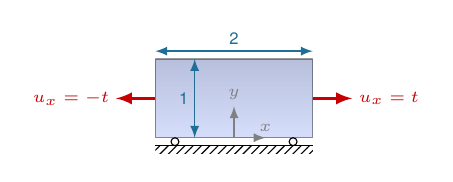
\begin{tikzpicture}[>=latex]

  % DOMAIN
  \path[domainstyle,domainshade] (-1.0, 0.0) rectangle (+1.0, +1.0);

  % DIMENSIONS
  \draw[dimension,<->] (-1.0, 1.1) -- (+1.0, 1.1) node[dimension,midway,above] {2};
  \draw[dimension,<->] (-0.5, 1.0) -- (-0.5, 0.0) node[dimension,midway,left] {1};

  % COORDINATE SYSTEM
  \draw[coordsys,->] (0.0, 0.0) -- (0.4, 0.0) node[coordsys,above] {$x$};
  \draw[coordsys,->] (0.0, 0.0) -- (0.0, 0.4) node[coordsys,above] {$y$};

  % BOUNDARY CONDITIONS
  \draw[dispbc,->] (+1.0, 0.5) -- (+1.5, 0.5) node[label,right] {$u_x = t$};
  \draw[dispbc,->] (-1.0, 0.5) -- (-1.5, 0.5) node[label,left] {$u_x = -t$};
  
  \draw (-0.75, -0.05) circle (0.05);
  \draw (+0.75, -0.05) circle (0.05);
  \draw[groundsurf] (-1.0, -0.1) -- (+1.0, -0.1);
  \path[ground] (-1.0, -0.2) rectangle (+1.0, -0.1);

\end{tikzpicture}
\end{center}

\begin{gather}
  u_x = \frac{v_x t}{l/2}, \quad v_x=1, \quad l=2. \quad w=1 \\
  \epsilon_{xx} = \frac{\partial u_x}{\partial x} + \frac{1}{2} \left( \frac{\partial u_x}{\partial x}\right)^2 \\
  \epsilon_{yy} = \frac{\partial u_y}{\partial y} + \frac{1}{2} \left( \frac{\partial u_y}{\partial y}\right)^2 
\end{gather}

\begin{gather}
  \sigma_{yy} = 0 \rightarrow \epsilon_{yy} = -\frac{\lambda}{\lambda+2\mu} \epsilon_{xx}
\end{gather}

\begin{gather}
  \text{Let \quad} e_y = \frac{\partial u_y}{\partial y} \\
  \epsilon_{yy} = e_y + \frac{1}{2} e_y^2 \\
  e_y = -1 + \sqrt{1 + 2\epsilon_{yy}}
\end{gather}

\begin{align}
  u_x = t x \\
  \epsilon_{xx} = t + \frac{1}{2} t^2 \\
  \epsilon_{yy} = -\frac{1}{3}(t + \frac{1}{2} t^2) \\
  e_y = -1 + \sqrt{1 - \frac{2}{3} (t + \frac{1}{2} t^2)} \\
  u_y = \left(-1 + \sqrt{1 - \frac{2}{3}t - \frac{1}{3}t^2}\right) y
\end{align}

\begin{align}
  S_{xx} &= \lambda(\epsilon_{xx} + \epsilon_{yy}) + 2\mu \epsilon_{xx} \\
  S_{xx} &= t + \frac{1}{2} t^2 -\frac{1}{3}(t + \frac{1}{2} t^2) + 2 (t + \frac{1}{2} t^2) \\
  S_{xx} &= \frac{1}{3}(4t^2 + 8t) \\
  S_{yy} &= 0
\end{align}

\begin{gather}
  \sigma_{xx} = S_{xx} \frac{X_{00}}{X_{11}} \\
  X_{00} = 1 + e_x = 1 + t \\
  X_{11} = 1 + ey = \sqrt{1 - \frac{2}{3}t - \frac{1}{3}t^2} \\
  \sigma_{xx} = S_{xx} \frac{1+t}{\sqrt{1 - \frac{2}{3}t - \frac{1}{3}t^2}} \\
  \sigma_{yy} = 0
\end{gather}





\end{document}



